\section{Deep Learning}
\label{section:introduction:deep-learning}
\subsection{An artificial neuron}
The fundamental building block of an artificial neural network is an artificial neuron.
\begin{definition}[neuron]
A \textbf{$d$-dimensional neuron} is a function $f_{\phi, \vec{w}, b} : \mathbb{R}^d \to \mathbb{R}$ of the form \begin{equation*}
    f_{\phi, \vec{w}, b} (x_1, \ldots, x_d) = \phi \left (\sum_{k=1}^d w_k x_k + b \right )
\end{equation*}
where $\phi : \mathbb{R} \to \mathbb{R}$, $\vec{w} \in \mathbb{R}^d$, $b \in \mathbb{R}$.
The vector $\vec{w}$ is known as the \textbf{weight vector} and its components $w_i$ are known as \textbf{weights}. The constant $b$ is known as a \textbf{bias} of the neuron. The function $\phi$ is known as an $\textbf{activation function}$.
\end{definition}
\begin{remark}
The function $f_{\phi, \vec{w}, b}$ is often expressed in the following matrix form
\begin{equation*}
    f_{\phi, \vec{w}, b} (\vec{x}) =  \phi (\langle \vec{w}, \vec{x} \rangle + b ) = \phi ( \vec{w}^\top \vec{x} + b ).
\end{equation*}
\end{remark}
\begin{remark}
We often want an activation function $\phi$ to be a function nonlinear in the input. The nonlinearity constraint plays an important role in the representation power of a single neuron and hence the neural network. Until recently, it was often imposed that $\phi$ is differentiable. Both of those constraints will be discussed in the upcoming sections. 
\end{remark}
\begin{figure}[h]
    \centering
    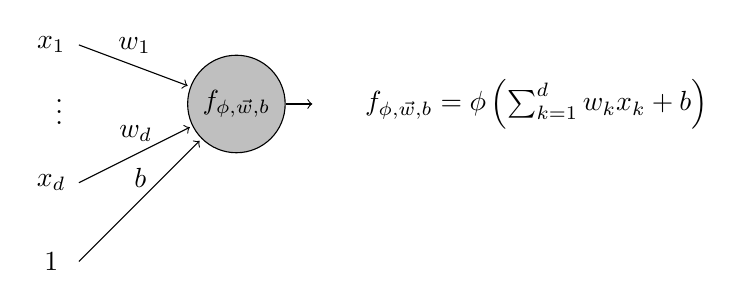
\begin{tikzpicture}[shorten >=1pt,->]
    	\tikzstyle{unit}=[draw,shape=circle,fill=black!25,minimum size=1.15cm]
    
    	\node[unit](p) at (2,1){$f_{\phi, \vec{w}, b}$};
    	\node(dots) at (-0.25,1){\vdots};
    
    	\draw (0,1.75) node[xshift=-10]{$x_1$} -- node[above=0.1em,align=center ] {$w_1$} (p);
    	\draw (0,0) node[xshift=-10]{$x_d$} -- node[above=0.1em,align=center ] {$w_d$} (p);
    	\draw (p) -- (3,1) node[xshift=80]{$f_{\phi, \vec{w}, b} = \phi \left (\sum_{k=1}^d w_k x_k + b \right )$};
    	\draw (0,-1) node[xshift=-10]{$1$} -- node[above=0.1em,align=center ] {$b$}  (p);

	\end{tikzpicture}
    \caption{A neuron parameterized with a weight vector $\vec{w}$, a bias $b$ and an activation function $\phi$. Addition of a bias parameter $b$ is often represented as a "virtual" input $1$ connected to the neuron with a weight of value $b$.}
    \label{fig:neuron}
\end{figure}
The structure and computation of an artificial neuron $f_{\phi, \vec{w}, b}$ is inspired by the structure of the biological neuron. Weights are inspired by synapses and the activation function $\phi$ is used to model the amount of information passed after the neuron processes the input. The model of an artificial neuron has no intention of emulating the much more complex biological counterpart. This analogy is visualized in Figure \ref{fig:neuron}. However, there is a strong connection between linear regression, logistic regression, and the single neuron. For more about linear regression and logistic regression, see Chapter 10 and Chapter 11 in \cite{pmlbook}.
\subsection{Activation functions}
\label{subsection:introduction:dl:activation-functions}
Commonly used activation functions include the logistic sigmoid ($\sigma$), rectified linear unit ($\operatorname{ReLU}$) and hyperbolic tangent ($\tanh$). Less commonly used is the hard binary threshold, also known as the Heaviside step function. However, there are many other activation functions and some of them were invented quite recently. Those include $\operatorname{PReLU}$\cite{he_2015_delving}, $\operatorname{SELU}$\cite{klambauer_2017_selfnormalizing}, $\operatorname{ELU}$\cite{clevert_2015_fast}, $\operatorname{PELU}$\cite{trottier_2018_parametric}. We will present the most commonly used activation functions.
\begin{definition}
The logistic sigmoid $\sigma : \R \to [0,1]$ is given by 
$\sigma(x) = \frac{1}{1 + \exp{(-x)}}$.
\end{definition}

\begin{definition}
The hyperbolic tangent $\tanh : \R \to [-1,1]$ is given by \newline $\tanh{(x)} = \frac{\exp{(x)} - \exp{(-x)}}{\exp{(x)} + \exp{(-x)}}$.
\end{definition}
\begin{definition}
The rectified linear unit $\operatorname{ReLU} : \R \to [0, \infty)$ is given by \newline $\operatorname{ReLU}(x) = \max{(0, x)}$.
\end{definition}
\begin{definition}
The Heaviside step function $s : \R \to \{0,1\}$ is given by
\[ 
    s(x) = \begin{cases} 
      1 & x > 0 \\
      0 & x \leq 0
   \end{cases}.
\]
\end{definition}
\begin{lemma}
\label{lemma:introduction:activation:sigmoid-derivative}
The logistic sigmoid is differentiable on $\R$. Moreover, its derivative satisfies $\frac{\partial \sigma}{\partial x} (x) = \sigma (x) \cdot (1 - \sigma(x)).$
\end{lemma}
\begin{proof}
Let $x \in \R$. Then $\frac{\partial \sigma}{\partial x} (x) = \frac{\exp{(-x)}}{(1 + \exp{(-x)})^2} = \sigma (x) \cdot (1 - \sigma (x)), \text{ as desired. }$
\end{proof}
\begin{figure}[H]
	\centering
	\subfigure[logistic sigmoid ($\sigma$)]{
    		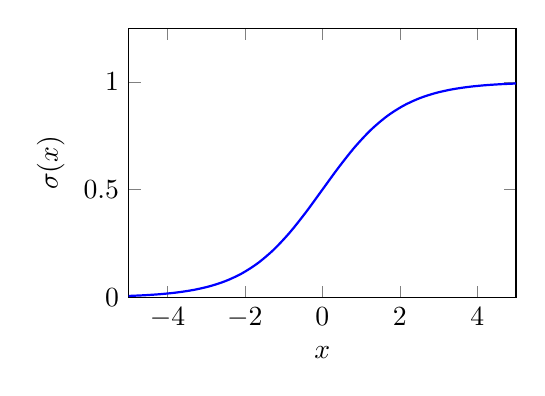
\begin{tikzpicture}
			\begin{axis}[width=6.5cm,height=5cm,ylabel=$\sigma(x)$,xlabel=$x$,ymin=0,ymax=1.25,xmin=-5,xmax=5]
				\addplot[thick,blue,smooth] {1/(1+exp(-x))};
			\end{axis}
		\end{tikzpicture}
	}
	\subfigure[hyperbolic tangent ($\tanh$)]{
		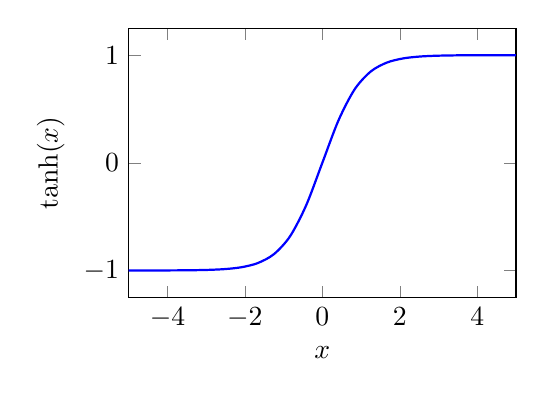
\begin{tikzpicture}
			\begin{axis}[width=6.5cm,height=5cm,ylabel=$\tanh(x)$,xlabel=$x$,ymin=-1.25,ymax=1.25,xmin=-5,xmax=5]
				\addplot[thick,blue,smooth] {tanh(x)};
			\end{axis}
		\end{tikzpicture}
	}\\
	\subfigure[rectified linear unit ($\operatorname{ReLU}$))]{
    		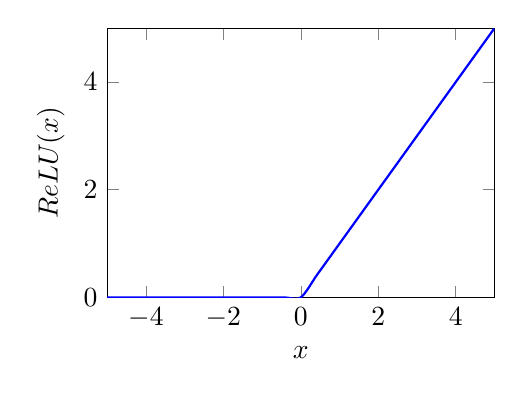
\begin{tikzpicture}
			\begin{axis}[width=6.5cm,height=5cm,ylabel=$\operatorname{ReLU}(x)$,xlabel=$x$,ymin=0,ymax=5,xmin=-5,xmax=5]
				\addplot[thick,blue,smooth] {max(0, x)};
			\end{axis}
		\end{tikzpicture}
	}
	\subfigure[Heaviside step function ($s$)]{
		\begin{tikzpicture}
			\begin{axis}[width=6.5cm,height=5cm,ylabel=$\operatorname{s}(x)$,xlabel=$x$,ymin=0,ymax=1.25,xmin=-5,xmax=5]
                \addplot[thick,blue,mark=*,samples at={-100,0}] {0};
                \addplot[thick,blue,mark=*,mark options={fill=white},samples at={0,100}] {1};
			\end{axis}
		\end{tikzpicture}
	}
    	\caption[Commonly used activation functions.]{Commonly used activation functions }
    	\label{fig:introduction:dl:activation-fns}
\end{figure}
\newpage
\subsection{A fully-connected layer}
To perform more complex computations, artificial neurons are often organized to form layers. The following definition will introduce the simplest form of a layer - a \textbf{fully-connected layer}. Many modern neural network layers can be very complex.
\begin{definition}[fully-connected layer]
\label{defn:layer}
A \textbf{fully-connected layer} is a function $f_{\phi, \vec{W}, \vec{b}} : \mathbb{R}^n \to \mathbb{R}^m$ of the form
\begin{equation*}
    f_{\phi, \vec{W}, \vec{b}} (x_1, \ldots, x_n) = \begin{bmatrix}
           f_{\phi, \vec{w_1}, b_1} (x_1, \ldots, x_n)  \\
           f_{\phi, \vec{w_2}, b_2} (x_1, \ldots, x_n) \\
           \vdots \\
           f_{\phi, \vec{w_m}, b_m} (x_1, \ldots, x_n)
         \end{bmatrix},
\end{equation*} where $\vec{W}$ is a matrix of weights corresponding to each neuron in the layer such that $\vec{W}_{i, j}$ is the weight connecting the $i$th input $x_i$ to $j$th neuron in the layer. For $1 \leq k \leq m$, we denote the weight vector of $k$th neuron in the layer by $\vec{w}_k$ and we denote the bias of $k$th neuron in the layer by $b_k$. Hence, weight vectors $\vec{w_1}, \ldots, \vec{w_m}$ are the columns of $\vec{W}$, and layer biases $b_1, \ldots, b_m$ are the components of the bias vector $\vec{b}$. The layer weight matrix $\vec{W}$ and the layer bias vector $\vec{b}$ are given by
\begin{equation*}
    \vec{W} = \begin{bmatrix}
    \vert & \vert  & \vert  & \vert \\
    \vec{w_1}   & \vec{w_2}  & \ldots  & \vec{w_m}   \\
    \vert & \vert & \vert  & \vert
    \end{bmatrix} \text{ and }
    \vec{b} = \begin{bmatrix}
       b_{1}  \\
       b_{2}  \\
       \vdots \\
       b_{m}
    \end{bmatrix}.
\end{equation*}
\end{definition}
\begin{figure}[H]
	\centering
    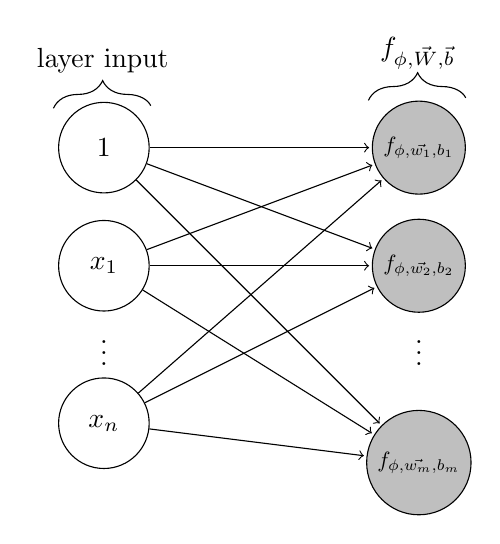
\begin{tikzpicture}[shorten >=1pt]
        \tikzstyle{unit}=[draw,shape=circle,minimum size=1.15cm, scale=0.8,fill=black!25]
        \tikzstyle{input}=[draw,shape=circle,minimum size=1.15cm]

        \node[input](x0) at (0,3.5){$1$};
        \node[input](x1) at (0,2){$x_1$};
        \node(dots) at (0,1){\vdots};
        \node[input](xd) at (0,0){$x_n$};
 
        \node[unit](y1) at (4,3.5){$f_{\phi, \vec{w_1}, b_1}$};
        \node[unit](y2) at (4,2){$f_{\phi, \vec{w_2}, b_2}$};
        \node(dots) at (4,1){\vdots};
        \node[unit](yc) at (4,-0.5){$f_{\phi, \vec{w_m}, b_m}$};
        
        \draw[->] (x0) -- (y1);
        \draw[->] (x0) -- (y2);
        \draw[->] (x0) -- (yc);
 
        \draw[->] (x1) -- (y1);
        \draw[->] (x1) -- (y2);
        \draw[->] (x1) -- (yc);
 
        \draw[->] (xd) -- (y1);
        \draw[->] (xd) -- (y2);
        \draw[->] (xd) -- (yc);
 
        \draw [decorate,decoration={brace,amplitude=10pt},xshift=-4pt,yshift=0pt] (-0.5,4) -- (0.75,4) node [black,midway,yshift=+0.6cm]{layer input};
        \draw [decorate,decoration={brace,amplitude=10pt},xshift=-4pt,yshift=0pt] (3.5,4.1) -- (4.75,4.1) node [black,midway,yshift=+0.6cm]{$f_{\phi, \vec{W}, \vec{b}}$};
    \end{tikzpicture}
    \caption[Network graph of a fully-connected layer with $n$-dimensional input units and $m$-dimensional output.]{A fully-connected layer with $n$-dimensional input and $m$-dimensional output, parameterized with a weight matrix $\vec{W}$, bias vector $\vec{b}$ and an activation function $\phi$. For the sake of clarity, weight and bias labels are omitted. }
    \label{fig:layer}
\end{figure}
\begin{remark}
The layer $f_{\phi, \vec{W}, \vec{b}}$ is often written in the more succint, matrix form
\begin{equation*}
    f_{\phi, \vec{W}, \vec{b}} (\vec{x}) = \phi(\vec{W}^\top \vec{x} + \vec{b}).
\end{equation*}
The application of $\phi$ is understood component-wise. 
\end{remark}
\begin{definition}
We define the \textbf{width} of a layer to be the number of neurons in the layer. Equivalently, the width of a layer is the dimension of the layer output.
\end{definition}
\subsection{A fully-connected neural network}
We are ready to introduce a fully-connected neural network, which is central to this thesis.
\begin{definition}[fully-connected neural network]
\label{defn:nn}
A \textbf{fully-connected neural network} of depth $L$ is a composition of $L$ fully-connected layers. Suppose that the first layer is a function $f_{\phi_1, \vec{W_1}, \vec{b_1}}^{(1)} : \mathbb{R}^{n_{(0)}} \to \mathbb{R}^{n_{(1)}}$ and the last layer is a function $f_{\phi_L, \vec{W_L}, \vec{b_L}}^{(L)} : \mathbb{R}^{n_{(L-1)}} \to \mathbb{R}^{n_{(L)}}$. Suppose that for $1 \leq k \leq L$, the $k$-th layer is a function $f_{\phi_k, \vec{W_k}, \vec{b_k}}^{(k)} : \mathbb{R}^{n_{(k-1)}} \to \mathbb{R}^{n_{(k)}}$. Now, a \textbf{fully-connected neural network} is a composite function parameterized by $L$ layer weight matrices $\{ \vec{W_k}  \}_{k=1}^{L}$, $L$ layer bias vectors $\{ \vec{b_k} \}_{k=1}^{L}$ and $L$ choices of layer activation functions $\{ \phi_{k} \}_{k=1}^{L}$ of the form
\begin{equation*}
    f = f_{\phi_L, \vec{W_L}, \vec{b_L}}^{(L)} \circ  f_{\phi_{(L-1)}, \vec{W_{(L-1)}}, \vec{b_{(L-1)}}}^{(L - 1)} \circ \ldots \circ f_{\phi_1, \vec{W_1}, \vec{b_1}}^{(1)}.
\end{equation*}
\end{definition}
\begin{figure}[H]
	\centering
	\begin{tikzpicture}[shorten >=1pt]
		\tikzstyle{unit}=[draw,shape=circle,minimum size=1.15cm]
		\tikzstyle{output}=[draw,shape=circle,minimum size=1.15cm,scale=0.9]
		\tikzstyle{hidden}=[draw,shape=circle,fill=black!25,minimum size=1.15cm]
 		\tikzstyle{lasthidden}=[draw,shape=circle,fill=black!25,minimum size=1.15cm,scale=0.8]

		\node[unit](x0) at (0,3.5){$1$};
		\node[unit](x1) at (0,2){$x_1$};
		\node at (0,1){\vdots};
		\node[unit](xd) at (0,0){$x_{n_{(0)}}$};
 
		\node[hidden](h10) at (3,4){$1$};
		\node[hidden](h11) at (3,2.5){$f_{1}^{(1)}$};
		\node at (3,1.5){\vdots};
		\node[hidden](h1m) at (3,-0.5){$f_{n_{(1)}}^{(1)}$};
 
		\node(h22) at (5,0){};
		\node(h21) at (5,2){};
		\node(h20) at (5,4){};
		
		\node(d3) at (6,0){$\ldots$};
		\node(d2) at (6,2){$\ldots$};
		\node(d1) at (6,4){$\ldots$};
 
		\node(hL12) at (7,0){};
		\node(hL11) at (7,2){};
		\node(hL10) at (7,4){};
		
		\node[hidden](hL0) at (9,4){$1$};
		\node[lasthidden](hL1) at (9,2.5){$f_1^{(L-1)}$};
		\node at (9,1.5){\vdots};
		\node[lasthidden](hLm) at (9,-0.5){$f_{n_{(L-1)}}^{(L-1)}$};
 
		\node[output](y1) at (12,3.5){$f_{1}^{(L)}$};
		\node[output](y2) at (12,2){$f_{2}^{(L)}$};
		\node at (12,1){\vdots};	
		\node[output](yc) at (12,0){$f_{n_{(L)}}^{(L)}$};
 
		\draw[->] (x0) -- (h11);
		\draw[->] (x0) -- (h1m);
 
		\draw[->] (x1) -- (h11);
		\draw[->] (x1) -- (h1m);
 
		\draw[->] (xd) -- (h11);
		\draw[->] (xd) -- (h1m);
 
		\draw[->] (hL0) -- (y1);
		\draw[->] (hL0) -- (yc);
		\draw[->] (hL0) -- (y2);
 
		\draw[->] (hL1) -- (y1);
		\draw[->] (hL1) -- (yc);
		\draw[->] (hL1) -- (y2);
 
		\draw[->] (hLm) -- (y1);
		\draw[->] (hLm) -- (y2);
		\draw[->] (hLm) -- (yc);
 
		\draw[->,path fading=east] (h10) -- (h21);
		\draw[->,path fading=east] (h10) -- (h22);
		
		\draw[->,path fading=east] (h11) -- (h21);
		\draw[->,path fading=east] (h11) -- (h22);
		
		\draw[->,path fading=east] (h1m) -- (h21);
		\draw[->,path fading=east] (h1m) -- (h22);
		
		\draw[->,path fading=west] (hL10) -- (hL1);
		\draw[->,path fading=west] (hL11) -- (hL1);
		\draw[->,path fading=west] (hL12) -- (hL1);
		
		\draw[->,path fading=west] (hL10) -- (hLm);
		\draw[->,path fading=west] (hL11) -- (hLm);
		\draw[->,path fading=west] (hL12) -- (hLm);
		
		\draw [decorate,decoration={brace,amplitude=10pt},xshift=-4pt,yshift=0pt] (-0.5,4) -- (0.75,4) node [black,midway,yshift=+0.6cm]{input layer};
		\draw [decorate,decoration={brace,amplitude=10pt},xshift=-4pt,yshift=0pt] (2.5,4.5) -- (3.75,4.5) node [black,midway,yshift=+0.6cm]{$1^{\text{st}}$ hidden layer};
		\draw [decorate,decoration={brace,amplitude=10pt},xshift=-4pt,yshift=0pt] (8.5,4.5) -- (9.75,4.5) node [black,midway,yshift=+0.6cm]{$(L-1)^{\text{th}}$ hidden layer};
		\draw [decorate,decoration={brace,amplitude=10pt},xshift=-4pt,yshift=0pt] (11.5,4) -- (12.75,4) node [black,midway,yshift=+0.6cm]{output layer};
	\end{tikzpicture}
	\caption[Network graph for a $(L+1)$-layer fully-connected neural network.]{Network graph of a $L$-layer fully-connected neural network with $n_{(0)}$-dimensional input and $n_{(L)}$-dimensional output. This illustration corresponds to Definition \ref{defn:nn}. The $k^{\text{th}}$ hidden layer contains $n_{(k)}$ neurons for $1 \leq k \leq L$. For the sake of clarity, parameters $\vec{W_k}, \vec{b_k}$ and activation functions $\phi_k$ are omitted from the graph. Hence, $f_{j}^{(k)}$ in the graph represents $(f_{\phi_k, \vec{W_k}, \vec{b_k}})_j$, in the sense of Definition \ref{defn:layer}.}
	\label{fig:nn}
\end{figure}
In literature, the layers $f_{\phi_k, \vec{W_k}, \vec{b_k}} : \mathbb{R}^{n_{(k-1)}} \to \mathbb{R}^{n_{k}}$, for $1 \leq k \leq L$ are often called $\textbf{hidden or latent layers}$. To analyse interactions between layers, we will often decompose $f_{\phi^{(k)}, \vec{W}^{(k)}, \vec{b}^{(k)}}$ into the computation of the affine transformation and the application of the activation function,  \begin{align*}
    f_{\phi^{(k)}, \vec{W}^{(k)}, \vec{b}^{(k)}} (\vec{x}) = \phi^{(k)} (\vec{a}^{(k)}(\vec{x})) \text{ where } \vec{a}^{(k)} (\vec{x})  = (\vec{W}^{(k)})^{\top}\vec{x} + \vec{b}^{(k)}.
\end{align*}
